\documentclass{exam}

\usepackage{units} 
\usepackage{graphicx}
\usepackage[fleqn]{amsmath}
\usepackage{cancel}
\usepackage{float}
\usepackage{mdwlist}
\usepackage{booktabs}
\usepackage{cancel}
\usepackage{polynom}
\usepackage{caption}
\usepackage{fullpage}
\usepackage{comment}
\usepackage{enumerate}
\usepackage{xfrac}

\newcommand{\dg}{\ensuremath{^\circ}} 
\everymath{\displaystyle}

\printanswers
\excludecomment{comment}

\ifprintanswers 
  \usepackage{2in1, lscape} 
\fi

\author{}
\date{November 13, 2013}
\title{Math 142 \\ Homework Eleven}

\begin{document}

  \maketitle

  \section{Homework}
  Section 6.5: 1-4, 9-21, 27-34, 37, 39-42, 46-49, 51

  \section{Extra Credit}
  Section 6.5: 35 and 36

  \ifprintanswers

    \begin{description}
      \item[35]
        The triangle formed has sides $a = 9$, $b = 10$, and $c = 11$.

        Use the Law of Cosines to find the angles in the triangle:
        \begin{align*}
          \angle A & \approx 50.48 \dg \\
          \angle B & \approx 58.99 \dg \\
          \angle C & \approx 70.53 \dg \\
        \end{align*}

        Convert to radians:
        \begin{align*}
          \angle A & \approx 0.8810 \\
          \angle B & \approx 1.030 \dg \\
          \angle C & \approx 1.231 \dg \\
        \end{align*}

        Find the areas of the three sectors:
        \begin{align*}
          A_1 & \approx \frac{1}{2} 0.881 \cdot 6^2 \\
              & \approx 15.858 \\
          \\
          A_2 & \approx \frac{1}{2} 1.03 \cdot 5^2 \\
              & \approx 12.875 \\
          \\
          A_3 & \approx \frac{1}{2} 1.231 \cdot 4^2 \\
              & \approx 9.848 \\
        \end{align*}

        Find the area of the triangle:
        \begin{align*}
          s  & = \frac{1}{2}(9 + 10 + 11) \\
             & = 15 \\
          \\
          A_{triangle} & = \sqrt{15 (15 - 9)(15 - 10) (15 - 11)} \\
                       & \approx 42.4264 \\
        \end{align*}

        The final area is the difference between the area of the triangle and the area of the three sectors:
        \begin{align*}
          Area & \approx 42.4264 - 15.858 - 12.875 - 9.848 \\
               & = \boxed{ \unit[3.85]{cm^2} } \\
        \end{align*}

    \end{description}

    \pagebreak
  \fi

  \section{Review}

  \begin{enumerate}
    \item What is the angle in degrees between the hour and minute hands of a clock at 12:20?

      \begin{solution}
        12:20 is one third of an hour past 12:00.  
        
        The hour hand has travelled one third of one twelfth of the way around:
        \[
          \angle H = \frac{1}{3} \cdot \frac{1}{12} \cdot 360 \dg = 10 \dg
        \]

        The minute hand has traveled one third of the way around:
        \[
          \angle M = \frac{1}{3} \cdot 360 \dg = 120 \dg
        \]

        The difference is:
        \[
          120 \dg - 10 \dg = 110 \dg
        \]

      \end{solution}

    \item Graph $f$.
      \[
        f(x) = 
        \begin{cases}
           \cos x  & \text{if } x < \pi \\
          - \sin x & \text{if } x >= \pi \\
        \end{cases}
      \]

      \begin{solution}
        \begin{figure}[H]
          \centering
          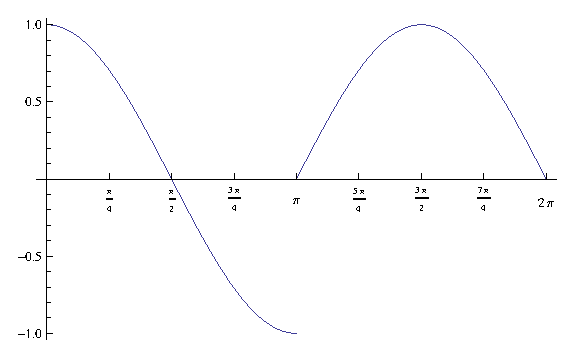
\includegraphics[scale=0.6]{review.eps}
          \caption{Review 2}
        \end{figure}
      \end{solution}

  \end{enumerate}

  \section{Section 6.5}

  \ifprintanswers

    \begin{description}

      \item[1] 
        \begin{align*}
          x^2 & = 21^2 + 42^2 - 2 \cdot 21 \cdot 42 \cdot \cos 39 \dg \\
          x   & \approx \boxed{ 28.88 } \\
        \end{align*}

      \item[2] 
        \begin{align*}
          x^2 & = 15^2 + 18^2 - 2 \cdot 15 \cdot 18 \cdot \cos 108 \dg \\
          x   & \approx \boxed{ 26.76 } \\
        \end{align*}

      \item[3] 
        \begin{align*}
          x^2 & = 25^2 + 25^2 - 2 \cdot 25 \cdot 25 \cdot \cos 140 \dg \\
          x   & \approx \boxed{ 46.98 } \\
        \end{align*}

      \item[4] 
        \begin{align*}
          x^2 & = 8^2 + 2^2 - 2 \cdot 8 \cdot 2 \cdot \cos 88 \dg \\
          x   & \approx \boxed{ 8.18 } \\
        \end{align*}

      \item[9] 
        \begin{align*}
          c^2 & = 10^2 + 18^2 - 2 \cdot 10 \cdot 18 \cdot \cos 120 \dg \\
          c   & \approx \boxed{ 24.58 } \\
          \\
          \cos A & \approx \frac{ 10^2 + 24.58^2 - 18^2}{2 \cdot 10 \cdot 24.58} \\
          A      & \approx \boxed{ 20.6 \dg }
          \\
          B & \approx 180 \dg - 120 \dg - 20.6 \dg \\
            & = \boxed{ 39.4 \dg } \\
        \end{align*}

      \item[10] 
        \begin{align*}
          \cos A & \approx \frac{ 12^2 + 44^2 - 12^2}{2 \cdot 12 \cdot 44} \\
          A      & \approx \boxed{ 63 \dg }
          \\
          \cos B & \approx \frac{ 40^2 + 44^2 - 12^2}{2 \cdot 40 \cdot 44} \\
          B      & \approx \boxed{ 15.5 \dg }
          \\
          C & \approx 180 \dg - 63 \dg - 15.5 \dg \\
            & = \boxed{ 101.5 \dg } \\
        \end{align*}

      \item[11]
        \begin{align*}
          c^2 & = 3.0^2 + 4.0^2 - 2 \cdot 3.0 \cdot 4.0 \cdot \sin 53 \dg \\
          c   & \approx \boxed{ 3.25 } \\
          \\
          \frac{\sin A}{3.0} &= \frac{\sin 53 \dg}{3.25} \\
          \angle A & \approx \boxed{ 47.5 \dg } \\
          \\
          \frac{\sin B}{4.0} &= \frac{\sin 53 \dg}{3.25} \\
          \angle B & \approx \boxed{ 79.5 \dg } \\
        \end{align*}

      \item[12]
        \begin{align*}
          a^2 & = 60^2 + 30^2 - 2 \cdot 60 \cdot 30 \cdot \sin 70 \dg \\
          a   & \approx \boxed{ 57.17 } \\
          \\
          \frac{\sin 70 \dg}{57.17} &= \frac{\sin B \dg}{60} \\
          \angle B & \approx \boxed{ 80.46 \dg } \\
          \\
          \frac{\sin 70 \dg}{57.17} &= \frac{\sin C \dg}{30} \\
          \angle C & \approx \boxed{ 29.54 \dg } \\
        \end{align*}

      \item[13]
        \begin{align*}
          \cos A &= \frac{25^2 + 22^2 - 20^2}{2 \cdot 22 \cdot 20} \\
          \angle A & \approx \boxed{ 49.87 } \dg \\
          \\
          \frac{\sin 49.87 \dg}{20} &= \frac{\sin B \dg}{25} \\
          \angle B & \approx \boxed{ 72.89 \dg } \\
          \\
          \frac{\sin 49.87 \dg}{20} &= \frac{\sin C \dg}{22} \\
          \angle C & \approx \boxed{ 57.25 \dg } \\
        \end{align*}

      \item[14]
        \begin{align*}
          \cos A   & = \frac{12^2 + 16^2 - 10^2}{2 \cdot 12 \cdot 16} \\
          \angle A & \approx \boxed{ 38.62 \dg } \\
          \\
          \frac{\sin 38.62 \dg}{10} &= \frac{\sin B \dg}{12} \\
          \angle B & \approx \boxed{ 48.51 \dg } \\
          \\
          \frac{\sin 38.62 \dg}{10} &= \frac{\sin C \dg}{16} \\
          \angle C & \approx \boxed{ 92.87 \dg } \\
        \end{align*}

      \item[15]
        solution one:
        \begin{align*}
          \frac{\sin 40 \dg}{125} & = \frac{\sin C}{162} \\
          C                       & \approx \boxed{ 56.4 } \dg \\
          A                       & \approx 180 \dg - 40 \dg - 56.4 \dg \\
                                  & \approx \boxed{ 83.6 } \dg
          \\
          \frac{\sin 40 \dg}{125} & = \frac{\sin 83.6 \dg}{a} \\
          a                       & \approx \boxed{ 193.2 } \\
        \end{align*}

        solution two:
        \begin{align*}
          \frac{\sin 40 \dg}{125} & = \frac{\sin C}{162} \\
          C                       & \approx \boxed{ 123.6 } \dg \\
          A                       & \approx 180 \dg - 40 \dg - 123.6 \dg \\
                                  & \approx \boxed{ 16.4 } \dg
          \\
          \frac{\sin 40 \dg}{125} & = \frac{\sin 16.4 \dg}{a} \\
          a                       & \approx \boxed{ 54.9 } \\
        \end{align*}

      \item[16]
        \begin{align*}
          \frac{\sin 52 \dg}{50} & = \frac{\sin A \dg}{65} \\
          \angle A               & \approx \boxed{ 78.97 \dg } \\
          \\
          \angle B & \approx 180 \dg - 78.97 \dg - 52 \dg \\
                   & = \boxed{ 49.03 \dg } \\
          \\
          \frac{\sin 52 \dg}{50} & = \frac{\sin 49.03 \dg}{b} \\
          b                      & \approx \boxed{ 52.18 } \\
        \end{align*}

      \item[17]
        \begin{align*}
          \frac{\sin 55 \dg}{50} &= \frac{\sin B}{65} \\
          \sin B &\approx 1.065 \\
        \end{align*}

        \fbox{No solution}

      \item[18]
        \begin{align*}
          A & = 180 \dg - 61 \dg - 83 \dg \\
            & = 36 \dg \\
          \\
          \frac{\sin 36 \dg}{73.5} & = \frac{\sin 83 \dg}{b} \\
          b                        & \approx \boxed{ 124.1 } \\
          \\
          \frac{\sin 36 \dg}{73.5} & = \frac{\sin 61 \dg}{c} \\
          c                        & \approx \boxed{ 109.4 } \\
        \end{align*}

      \item[19]
        \begin{align*}
          B & = 180 \dg - 85 \dg - 35 \dg \\
            & = 60 \dg \\
            \\
          \frac{\sin 60 \dg}{3} & = \frac{\sin 35 \dg}{x} \\
          x                     & \approx \boxed{ 1.99 } \\
        \end{align*}

      \item[20]
        \begin{align*}
          x^2 & = 10^2 + 18^2 - 2 \cdot 10 \cdot 18 \cdot \cos 40 \dg \\
              & \approx \boxed{ 25.77 } \\
        \end{align*}

      \item[21]
        \begin{align*}
          \frac{\sin 100 \dg}{50} & = \frac{\sin 30 \dg}{x} \\
          x                       & \approx \boxed{ 25.4 } \\
        \end{align*}

      \item[27]
        \begin{align*}
          s  & = \frac{1}{2}(9 + 12 + 15) \\
             & = 18 \\
          \\
          A  & = \sqrt{18 (18 - 9)(18 - 12) (18 - 15)} \\
             & = \boxed{ 54 } \\
        \end{align*}

      \item[28]
        \begin{align*}
          s  & = \frac{1}{2}(1 + 2 + 2) \\
             & = 2.5 \\
          \\
          A  & = \sqrt{2.5 (2.5 - 1)(2.5 - 2) (2.5 - 2)} \\
             & \approx \boxed{ 0.9682 } \\
        \end{align*}

      \item[29]
        \begin{align*}
          s  & = \frac{1}{2}(7 + 8 + 9) \\
             & = 12 \\
          \\
          A  & = \sqrt{12 (12 - 7)(12 - 8) (12 - 9)} \\
             & \approx \boxed{ 26.83 } \\
        \end{align*}

      \item[30]
        \begin{align*}
          s  & = \frac{1}{2}(11 + 100 + 101) \\
             & = 106 \\
          \\
          A  & = \sqrt{106 (106 - 11)(106 - 100) (106 - 101)} \\
             & \approx \boxed{ 549.64 } \\
        \end{align*}

      \item[31]
        \begin{align*}
          s  & = \frac{1}{2}(4 + 3 + 6) \\
             & = 6.5 \\
          \\
          A  & = \sqrt{6.5 (6.5 - 4)(6.5 - 3) (6.5 - 6)} \\
             & \approx \boxed{ 5.33 } \\
        \end{align*}

      \item[32]
        Find the area of one of the two identical triangles:
        \begin{align*}
          s  & = \frac{1}{2}(5 + 5 + 2) \\
             & = 6 \\
          \\
          A  & = \sqrt{6 (6 - 5)(6 - 5) (6 - 2)} \\
             & \approx 4.899 \\
        \end{align*}

        Since there are two triangles, the total area is twice the area of one triangle: 
        \[
          A_{total} = 2 \cdot 4.99 \approx \boxed{ 9.798 }
        \]

      \pagebreak

      \item[33]
        Draw a diagonal from left to right in the figure to form two triangles.  Then use the Law of Cosines to find the
        length of the diagonal:
        \begin{align*}
          a^2 & = 5^2 + 6^2 - 2 \cdot 5 \cdot 6 \cdot \cos 100 \dg \\
          a   & \approx 8.45 \\
        \end{align*}

        Find the area of the top triangle:
        \begin{align*}
          s_1 & = \frac{1}{2}(5 + 6 + 8.45) \\
              & = 9.725 \\
          \\
          A_1 & = \sqrt{9.725 (9.725 - 5)(9.725 - 6) (9.725 - 8.45)} \\
              & \approx 14.77 \\
        \end{align*}

        Find the area of the bottom triangle:
        \begin{align*}
          s_1 & = \frac{1}{2}(8 + 7 + 8.45) \\
              & = 11.72 \\
          \\
          A_2 & = \sqrt{11.72 (11.72 - 8)(11.72 - 7) (11.72 - 8.45)} \\
              & \approx 26.00 \\
        \end{align*}

        The total area is: 
        \[
          A_{total} \approx 14.77 + 26.00 = \boxed{ 40.77 }
        \]

      \item[34]
        If you split the $60 \dg$ angle in half, you get two identical triangles which each contain a $30 \dg$ angle.

        Use the Law of Sines to find another angle:
        \begin{align*}
          \frac{\sin 30 \dg}{3} & = \frac{\sin A}{4} \\
          A                     & \approx 41.82 \dg \\
        \end{align*}

        Since $\angle A > 90 \dg$ in the figure, $A = 90 \dg + 41.82 \dg = 131.82 \dg$.

        The remaining angle is:
        \[
          B = 180 \dg - 131.82 \dg - 30 \dg = 18.18 \dg
        \]

        Use the Law of Sines to find the missing side:
        \begin{align*}
          \frac{\sin 30 \dg}{3} & = \frac{\sin 18.18}{b} \\
          b                     & \approx 1.872 \\
        \end{align*}

        Find the area of one triangle:
        \begin{align*}
          s  & = \frac{1}{2}(4 + 3 + 1.872) \\
             & = 4.436 \\
          \\
          A  & = \sqrt{4.436 (4.436 - 4)(4.436 - 3) (4.436 - 1.872)} \\
             & \approx 2.67 \\
        \end{align*}

        Multiply by two to get the total area:
        \[
          A_{total} \approx 2 \cdot 2.67 = \boxed{ 5.337 }
        \]

      \item[37]
        Use the Law of Cosines:
        \begin{align*}
          c^2 & = 2.82^2 + 3.56^2 - 2 \cdot 2.82 \cdot 3.56 \cdot \cos 40.3 \dg \\
          c   & \approx \boxed{ \unit[2.30]{mi} } \\
        \end{align*}

      \pagebreak

      \item[39]
        First find out how far each car has travelled in the 30 minutes they've been driving:
        \begin{align*}
          d_1 &= 0.5 \cdot 50 = \unit[25]{mi} \\
          d_2 &= 0.5 \cdot 30 = \unit[15]{mi} \\
        \end{align*}

        Use the Law of Cosines to figure out how far apart they are:
        \begin{align*}
          d^2 & = 25^2 + 15^2 - 2 \cdot 25 \cdot 15 \cdot \cos 65 \dg \\
          d   & \approx \boxed{ \unit[23.1]{mi} } \\
        \end{align*}

      \item[40]
        The car travelled east for 40 miles and northeast for 20 miles.  The angle between the two sides is:
        \[
          \angle A = 90 \dg + 45 \dg = 135 \dg
        \]

        Use the Law of Cosines to find the distance:
        \begin{align*}
          d^2 & = 40^2 + 20^2 - 2 \cdot 40 \cdot 20 \cdot \cos 135 \dg \\
          d   & \approx \boxed{ \unit[56]{mi} } \\
        \end{align*}

      \item[41]
        Find the distances travelled on each leg of the trip:
        \begin{align*}
          d_1 &= 1.5 \cdot 625 = \unit[937.5]{mi} \\
          d_2 &= 2 \cdot 625 = \unit[1250]{mi} \\
        \end{align*}

        The angle is slightly less than $180 \dg$:
        \[
          \angle A = 180 \dg - 10 \dg = 170 \dg
        \]

        Use the Law of Cosines to find the distance:
        \begin{align*}
          d^2 & = 937.5^2 + 1250^2 - 2 \cdot 937.5 \cdot 1250 \cdot \cos 170 \dg \\
          d   & \approx \boxed{ \unit[2179]{mi} } \\
        \end{align*}

      \item[42]
        After one hour, the first boat has travelled 30 miles and the second boat has travelled 26 miles.

        The angle is:
        \[
          \angle A = 180 \dg - 50 \dg - 70 \dg = 60 \dg
        \]

        Use the Law of Cosines to find the distance:
        \begin{align*}
          d^2 & = 30^2 + 26^2 - 2 \cdot 30 \cdot 26 \cdot \cos 60 \dg \\
          d   & \approx \boxed{ \unit[28]{mi} } \\
        \end{align*}

      \item[46]
        \begin{align*}
          \cos A & = \frac{230^2 + 212^2 - 120^2}{2 \cdot 230 \cdot 212} \\
          A      & \approx 31.2 \dg \\
        \end{align*}

      \item[47]
        \begin{align*}
          d^2 & = 380^2 + 420^2 - 2 \cdot 380 \cdot 420 \cdot \cos 30 \dg \\
          d   & \approx \boxed{ \unit[211]{ft} } \\
        \end{align*}

      \item[48]
        The angle between the tower and the hill is:
        \[
          \angle A = 90 \dg + 32 \dg = 120 \dg
        \]

        Use the Law of Cosines to find the length:
        \begin{align*}
          L^2 & = 125^2 + 55^2 - 2 \cdot 125 \cdot 55 \cdot \cos 32 \dg \\
          L   & \approx \boxed{ \unit[83.6]{ft} } \\
        \end{align*}

      \pagebreak

      \item[49]
        If $x$ is the distance from the base of the mountain to the center:
        \begin{align*}
          \tan 74 \dg & = \frac{3400}{x} \\
          x           & \approx \unit[974.93]{ft} \\
        \end{align*}

        The cable length is the hypotenuse of the large right triangle:
        \begin{align*}
          L^2 &= (800 + 974.93)^2 + 3400^2 \\
          L &\approx \boxed{ \unit[3835]{ft} } \\
        \end{align*}

      \item[51]
        Find the area:
        \begin{align*}
          s & = \frac{1}{2} (112 + 148 + 190) \\
            & = 225 \\
          \\
          A & = \sqrt{225 (225 - 112)(225 - 148) (225 - 190)} \\
            & \approx \unit[8278]{ft^2} \\
        \end{align*}

        Find the value:
        \[
          value = \unit[20]{dollars/ft^2} \cdot \unit[8278]{ft^2} = \boxed{ \$165,554 }
        \]

    \end{description}

  \else
    \vspace{1 cm}
    \begin{quote}
      \begin{em}
        TO DO
      \end{em}
    \end{quote}
    \hspace{1 cm} --Source
  \fi

\end{document}

